% Copyright \copyright\ 2013  Simon Kalt, Jan-Peter Hohloch, Tobias Fabritz
% Es wird die Erlaubnis gegeben, dieses Dokument unter den Bedingungen der von der Free
% Software Foundation veröffentlichen  GNU Free
% Documentation License (Version 1.2 oder neuer) zu kopieren, verteilen und/oder
% zu verändern. Eine Kopie dieser Lizenz ist unter
% http://www.gnu.org/copyleft/fdl.txt erhältlich.
%
% Zusätzlich muss jede Kopie/Aktualisierung wieder über die Seite
% der Fachschaft Informatik der Uni Tübingen
% den Studenten zur Verfügung gestellt werden
% http://www.fsi.uni-tuebingen.de/

\chapter{Graphen}
    \section{Definition}
        Ein Graph sei definiert durch $G=(V,E)$ wobei $V$ (Vertices) eine endliche Menge von Knoten sei und $E \subseteq V \times V$ (Edges) eine endliche Menge von Kanten. Dabei heißt $e=(v,w) \in E$ Kante von $v$ nach $w$ und $w$ heißt Nachbarknoten von $v$ (adjazent). Ein \emph{Pfad} in $G$ ist eine Folge $(v_0,v_1,...,v_k)$ von Kanten mit $k \geq 0$ und $(v_i,v_{i+1} \in E \ \forall \ 0 \leq i \leq k-1$ (Pfad von $v_0$ nach $v_k$). Falls $v_0 = v_k$ und $k \geq 1$ heißt der Pfad Zykel. Falls $v_i \neq v_j$ für $i \neq j$ heißt der Pfad einfach. Wir schreiben
     
        $$
            v \overset{*}{\rightarrow_{G}} w 
        $$
        für einen Pfad von $v$ nach $w$. Der Graph heißt \emph{zyklisch} falls er Zykel enthält, sonst \emph{azyklisch}. $G$ heißt \emph{Baum}, falls
        \begin{enumerate}[a)]
            \item $V$ enthält genau ein $v_0$ mit $\text{inadj}(v_0) = 0$
            \item $\forall v \in V \backslash \{v_0\} : \text{inadj(v)}=1$
            \item G ist azyklisch
        \end{enumerate}
        
        \section{Darstellung von Graphen}            
            \subsection{Darstellung im Computer}
                Wir nehmen an, dass $V=\{1,2,...,n\}$. Dann ergeben sich die Darstellungen
                \begin{enumerate}
                    \item Darstellung: \emph{Adjazenzmatrix A}. Dabei gilt in der Matrix
                        $$
                            a_{i,j} \begin{cases}
                                        1 & \text{falls} (i,j) \in E \\
                                        0 & \text{sonst}
                                    \end{cases}
                        $$
                        wobei diese Matrix in einem ungerichteten Graphen symmetrisch ist. Dabei verbraucht die Matrix einen Platz von $\LO(n^2)$. Dies ist gut, falls $\abs{E} = m$ ungefähr so groß ist wie $n^2$.
                    \item Darstellung: \emph{Adjazenzlisten}. Dabei wird für jedes $v$ die Knotenmenge gespeichert: Dabei ist
                        $$
                            \text{Out: adj}(v) = \{ w \in V | (v,w) \in E \}
                        $$
                        und
                        $$
                            \text{Inadj}(v) = \{ w \in V | (w,v) \in E \}
                        $$
                        Für ungerichtete Graphen ergibt sich
                        $$
                            \text{Outadj}(v) = \{ w \in V | (v,w) \in E \}
                        $$     
                        Dabei haben wir einen Platzverbrauch von $\LO(n+m)$. Als Nachteil ergibt sich beim Zugrif auf Kante $(v,w)$ kostet $\LO(addj(v))$ wobei
                        $$
                            \text{addj}(v) = \abs{\{w \in V | (v,w) \in E \}}
                        $$        
                \end{enumerate}
                
            \subsubsection{Beispiel}
            %%%%%%%%%%%%%%%%%
            % Hier Skizze und Liste noch einfügen, evtl noch baum skizze
            %%%%%%%%%%%%%%%%%
                Sei $G = (V, E)$ mit $V= \{1,2,3,4,5\}$ und $E=\{(1,2),(1,3),(1,4),(4,5),(5,1),(3,5)\}$. Für $G$ ergibt sich die folgende Adjazenzmatrix:
                $$
                    \begin{array}{c|ccccc}
                    - & 1 & 2 & 3 & 4 & 5 \\ 
                    \hline
                    1 & 0 & 1 & 1 & 1 & 0 \\ 
                    2 & 0 & 0 & 0 & 0 & 0 \\ 
                    3 & 0 & 0 & 0 & 0 & 1 \\ 
                    4 & 0 & 0 & 0 & 0 & 1 \\ 
                    5 & 1 & 0 & 0 & 0 & 0
                    \end{array} 
                $$
                Der zugehörige Graph ist in \autoref{fig:directed-graph} dargestellt.
                \begin{figure}[htp]
                    \capstart
                    \centering
                    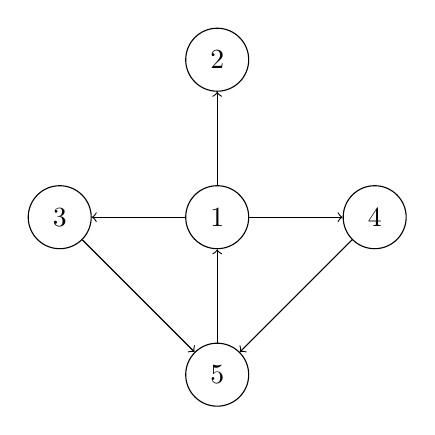
\begin{tikzpicture}[->,every node/.style={shape=circle, draw, minimum size=8mm},node distance=2cm]
    \node (1) {1};
    \node (2) [above of=1] {2};
    \node (3) [left of=1] {3};
    \node (4) [right of=1] {4};
    \node (5) [below  of=1] {5};

    \path (1) edge (2)
          (1) edge (3)
          (1) edge (4)
          (3) edge (5)
          (4) edge (5)
          (5) edge (1);
\end{tikzpicture}
                    \caption{Gerichteter Graph $G = (V, E)$}
                    \label{fig:directed-graph}
                \end{figure}      

            \section{Topologisches Sortieren}
                Sei $G=(V,E)$ ein gerichteter Graph (Digraph). Abbildung 
                $$
                    \text{num: } V \rightarrow \{1,2,...,n \}
                $$
                und $n= \abs{V}$ heißt topologische Sortierung falls für alle $(v,w) \in E$ gilt
                $$
                    \text{num}(v) < \text{num}(w)
                $$
                \begin{satz}
                    Die Abbildung \emph{num} existiert genau für azyklische Graphen
                \end{satz}
                
                \begin{proof}
                    \begin{itemize}
                        \item $\Rightarrow$: Annahme $G$ zyklisch. Sei $(V_0,...,v_k = v_0)$ ein Zykel. Es muss gelten: 
                        $$
                            \text{num}(v_0) < \text{num}(v_1) < ... < \text{num}(v_k) = \text{num}(v_0)
                        $$
                        Dies ist ein Widerspruch.
                        \item $\Leftarrow$: Sei $G$ azyklisch. Behauptung: $G$ enthält Knoten mit $\text{indeg} = 0$ (Anzahl eingehender Kanten)
                            \begin{proof}
                                Induktion über Größe von $V$. Für $\abs{V} = 1$ trivial. Für $\abs{V} > 1$: Entferne beliebigen Knoten $v \in V$. Dann erhalte ich damit $G' = (V,E')$ mit $V' = V \backslash \{v\}$ und $E' = E \cap (V' \times V')$. Nach Induktionsannahme ist $G'$ azyklisch und enthält Knoten $v'$ mit $\text{indeg}(v') = 0$. Entferne $v'$ aus $G'$ und erhalte $G''$. $G''$ enthält auch wieder ein $v''$ mit $\text{indeg}(v'')=0$. Lese den Beweis nochmal, wobei als $v$ nun $v''$ gewählt ist. Entweder ist $\text{indeg}(v')=0$ in $G$ oder $\text{indeg}(v'') = 0$ in $G$, denn es können nicht beide Knoten $(v',v'')$ und $(v'',v')$ in $E$ existieren wegen Zykelfreiheit.
                            \end{proof}
                    \end{itemize}
                \end{proof}
                
                \subsection{Algorithmus}
                    Beschreibung (\autoref{alg:topologischesSortieren}):
                    \begin{itemize}
                        \item $\abs{V}=1$ trivial
                        \item $\abs{V} > 1$: Wähle v mit $\text{indeg}(v)=0$, entferne dann $v$ und erstelle rekursiv $G'$
                            Sei $\text{num': } V' \rightarrow \{1,...., \abs{V'}\}$ Dann ist num für G:
                            $$
                                \text{num}(w) = \begin{cases}
                                                    \text{num}'(w) + 1 & \text{falls } w \neq v \\
                                                    1 & \text{sonst}
                                                \end{cases}
                            $$                          
                    \end{itemize}
                    
                    \begin{algorithm}
                    	\caption{Topologisches Sortieren}
                    	\label{alg:topologischesSortieren}
                    	\begin{algorithmic}
                    		\State count $\gets$ 0
                    		\While{$\exists v\in V:indeg(v)=0$}
                    			\State count $\gets$ count$ +1$
                    			\State num(v) $\gets$ count
                    			\State streiche v und ausgehende Kanten
                    		\EndWhile
                    		\If{count$ < |V|$}
                    			G zyklisch
                    		\EndIf
                    	\end{algorithmic}              
                    \end{algorithm}
                    
                    
%                    \begin{verbatim}
%                        count <- 0
%                        while exists v aus V mit indeg(v) = 0 do
%                            count++
%                            num(v) <- count
%                            streiche v und ausgeh. Kanten
%                        od
%                        if count < |V| 
%                        then G zyklisch
%                    \end{verbatim}


                    Dabei ergeben sich als Kosten $\LO(n+m)$ für die Zeit und den Platzverbrauch, wobei $\abs{V} = n, \abs{E}=m$. Dabei werden Adjazenzlisten benutzt, da sonst der Platz quadratisch wäre. Außerdem brauchen wir ein Array \emph{indeg}, welches die Zahl der eingehenden Kanten zählt.
                    (\autoref{fig:topSort})
                    
										
					\begin{figure}[htp]
						\capstart
						\centering
						
\begin{tikzpicture}[-, >=stealth', auto, node distance=1cm]
   %Outadjazenzliste:
	 \node[rectangle,draw] (out1) {1};
		 \node[circle,draw] (out12) [right of=out1] {2};
		 \node[circle,draw] (out13) [right of=out12] {3};
	 	 \node[circle,draw] (out14) [right of=out13] {4};
		 \node[circle,draw] (out17) [right of=out14] {7};
		
	 \node[rectangle,draw] (out2) [below of=out1] {2};
	     \node[circle,draw] (out21) [right of=out2] {6};
		\node[circle,draw] (out26) [right of=out21] {7};
			
	\node[rectangle,draw] (out3) [below of=out2] {3};
	    \node[circle,draw] (out34) [right of=out3] {4};
		
	 \node[rectangle,draw](out4)[below of=out3]{4};
	    \node[circle,draw](out45)[right of=out4]{5};
			
	 \node[rectangle,draw](out5)[below of=out4]{5};
		\node[circle,draw](out56)[right of=out5]{6};
		\node[circle,draw](out57)[right of=out56]{7};
    
	 \node[rectangle,draw](out6)[below of=out5]{6};
	
	 \node[rectangle,draw](out7)[below of=out6]{7};
	 
	 
	 \node (map) [right of=out17] {$\mapsto$};
%Indegree:
   
	 \node[rectangle,draw] (in1) [right of=map] {1};
	 	\node (ind1) [right of=in1] {0};
		
	 \node[rectangle,draw] (in2) [below of=in1] {2};
	 	\node (ind2) [right of=in2] {I};
			
	\node[rectangle,draw] (in3) [below of=in2] {3};
	 	\node (ind3) [right of=in3] {I};
		
	 \node[rectangle,draw](in4)[below of=in3]{4};
	 	\node (ind4) [right of=in4] {II};
			
	 \node[rectangle,draw](in5)[below of=in4]{5};
	 	\node (ind5) [right of=in5] {I};
    
	 \node[rectangle,draw](in6)[below of=in5]{6};
	 	\node (ind6) [right of=in6] {II};
	
	 \node[rectangle,draw](in7)[below of=in6]{7};
	 	\node (ind7) [right of=in7] {III};
	 	
	 	
	 %Text:
	 \node (Outadj) [above of=out1] {Outadj:};
	 \node (Indeg) [above of=in1] {Indeg:};
	
	\path[draw]
		 (out1) edge (out2)
		 (out2) edge (out3)
		 (out3) edge (out4)
		 (out4) edge (out5)
		 (out5) edge (out6)
		 (out6) edge (out7)
		
		 (out1) edge (out12)
		 (out12) edge (out13)
		 (out13) edge (out14)
		 (out14) edge (out17)
		
		 (out2) edge (out21)
		 (out21) edge (out26)
		
		 (out3) edge (out34)
		
		 (out4) edge (out45)
		
		 (out5) edge (out56)
		 (out56) edge (out57);
	
	\path[draw]
		 (in1) edge (in2)
		 (in2) edge (in3)
		 (in3) edge (in4)
		 (in4) edge (in5)
		 (in5) edge (in6)
		 (in6) edge (in7);
		 
\end{tikzpicture}

						\label{fig:topSort}
						\caption{Beispiel zum topologischen Sortieren}
					\end{figure}
                    
                    
            \section{Billigste Wege}
                Gegeben sei ein Netzwerk $(V,E,c)$ mit $G=(V,E)$ und $c: E \rightarrow \R$
                
								\begin{figure}
									\centering
									\begin{tikzpicture}[->,node distance=3cm]
  \node[state] (1) {1};
	\node[state] (2) [above right of=1] {2};
	\node[state] (3) [right of=1] {3};
	\node[state] (4) [right of=2] {4};
	\node[state] (5) [right of=3] {5};
	
	\path
			(1) edge node[above left]{2} (2)
			(1) edge[bend right] node[below]{3} (3)
			
			(2) edge node[right]{-3} (3)
			(2) edge node[above]{-1} (4)
			
			(3) edge[bend right] node[above]{-1} (1)
			(3) edge node[below]{1} (5)
			(3) edge node[right]{2} (4)
			
			(4) edge node[right]{3} (5);
\end{tikzpicture}
									\caption{Graph mit Pfadkosten (negativer Zykel)}
								\end{figure}
                Ziel ist es den Pfad mit den geringsten Kosten zwischen zwei gegebenen Knoten zu finden. Dabei sind die Kosten eines Pfades $p= v_0,...,v_k$  gegeben durch 
                $$
                    c(p) = \sum_{i=0}^{k-1}{c((v_i,v_{i+1}))}
                $$
                Dabei unterscheiden wir folgende Probleme
                \begin{enumerate}
                    \item Single source - single sink shortest path
                    \item single source shortest path
                    \item all pairs shortest path
                \end{enumerate}
                
           \subsection{Single source shortest path}
                    Für $u \in V$ sei $P(s,u)$ die Menge aller Pfade von $s$ nach $u$. Wir definieren als Kosten
                    $$
                        \delta(u) = \begin{cases}
                                            \infty & \text{falls } P(s,u) = \emptyset \\
                                            \inf\{c(p) | p \in P(s,u)\} & \text{sonst}
                                        \end{cases}
                    $$ 
                    Ein negativer Zykel $p$ hat dabei $c(p) < 0$.
                    \begin{lemma}
                        Sei $u \in V$ Dann
                        \begin{enumerate}[i)]
                            \item $\delta(u) = -\infty$ gdw. u erreichbar über negativen Zykel, der von $s$ aus erreichbar ist.
                            \item $\delta(v) \in \R$: Es existiert ein billigster Weg von $s$ nach $u$ mit Kosten $\delta(u)$
                        \end{enumerate}
                    \end{lemma}
                    \begin{proof}
                        \begin{enumerate}[i)]
                            \item   \begin{itemize}
                                        \item $\Rightarrow$: trivial
                                        \item $\Leftarrow$: Sei $C= \sum_{i \in E}{\abs{c(e)}}$ und sei $p$ ein billigster Weg von $s$ nach $n$ mit $c(p) < -C$. Es folgt, dass $p$ einen negativen Zykel enthalten muss.
                                    \end{itemize}   
                            \item $\delta(u) < \infty$, d.h. es gibt Pfad von $s$ nach $u$. Es wird nun Behauptet, dass 
                            $$
                                \delta(u) = \min\{c(p) | p \in P(s,u) \text{ und p einfach}\}
                            $$
                                \begin{proof}
                                    Sei $p'$ ein billigster, einfacher Weg von $s$ nach $u$. Ist die Behauptung falsch, so gibt es einen nicht einfachen Weg $q$ mit $c(q) < c(p')$. Da es keine negativen Zykel gibt gilt: Durch Wegnahme des Zykels aus $q$ entsteht ein billigerer Weg $q'$ mit $c(q') \leq c(q) < c(p')$. Dies ist ein Widerspruch.
                                \end{proof}                                                             
                        \end{enumerate}
                    \end{proof}
                    
                \paragraph{Beispiel}
								    %TODO : sinnvolle Aufteilung der Fälle
                    \emph{1. Fall}: $G$ ist azyklisch. Wir nehmen an, dass $G$ topologisch sortiert ist.  Dann ergibt sich als Algorithmus
                    
                    \begin{algorithm}
                    	\caption{Single Source Shortest Path --- Graph azyklisch}
                    	\label{alg:sssp1}
                    	\begin{algorithmic}
                    		\State d(s) $\gets$ 0, Pfad(s) $\gets$ s
                    		\State d(v) $\gets \infty \forall v\in V\backslash \set{s}$
                    		\For{$i\gets s+1$ to $n$}
                    			\State d(v) $\gets \min_u\set{d(n)+c((u,v)) | (u,v)\in E}$
                    			\State Pfad(v) $\gets$ Pfad(u*) + v \Comment Konkatenation
                    		\EndFor
                    	\end{algorithmic}
                    \end{algorithm}
                    
%                    \begin{verbatim}
%d(s) <- 0, Pfad(s) <- s
%d(v) <- infty für alle v \in V \ {s}
%for i <- s+1 to n do
%    d(v) <- min_u{d(n) + c((u,v)) | (u,v) \in E }
%    Pfad(v) <- Pfad(u*) + v // konkateniere
%od
%                    \end{verbatim}

                % Vorlesung 18. Juni
            \subsection{Dijkstra's Algorithmus}
						%TODO : s.o.
						\emph{2. Fall}: Kanten in G haben nur positive Kosten, Zykel erlaubt\\
            Gegeben ein Graph $G = (V, E)$ und eine Kostenfunktion $c: E \to \R^+$.
            Weiterhin zwei Mengen $S, S'$ mit Source $s \in S$. Hierbei ist $S$ die Menge der Knoten $u \in V$ mit bekanntem $\delta(u)$. $S'$ ist die Menge der Knoten aus $V \setminus S$, die Nachbarn in $S$ haben.

            \begin{algorithm}
            	\capstart
            	\caption{Dijkstra's Algorithmus}
            	\begin{algorithmic}
            		\State $S\gets \{s\}$
            		\State $d(s)\gets 0$
            		\State $S'\gets$ \Call{Out}{S} \Comment Knoten welche von S aus direkt erreichbar sind
            		\State $d'(u)\gets c((s,u)) \forall u\in S'$
            		\State $d'(u)\gets \infty \forall u\in V\backslash \left(S\cup S'\right)$
            		\While{$S\not= V$}
            			\State wähle $w\in S'$ mit geringstem $d'(w)$
            			\State $d(w)\gets d'(w)$
            			\State $S\gets S\cup \{w\}$
            			\ForAll{$u\in$ \Call{OUT}{w}}
            				\If{$u\not\in S$}
            					\State $S'\gets S'\cup \{u\}$\Comment falls bereits zuvor $u\in S'$ kein Unterschied
            					\State $d'(u)\gets \min\{d'(u),d(w)+c(w,u)\}$
            				\EndIf
            			\EndFor
            		\EndWhile
            	\end{algorithmic}
            	\label{alg:Dijkstras}
            \end{algorithm}
            
%            \begin{verbatim}
%S <- {s}, d(s) <- 0
%S' <- Out(s) // (Knoten welche von S aus direkt erreichbar sind)
%d'(u) < c((s,u)) für alle u \in S'
%d'(u) <- \infty für alle u \in V\{S \cup S'}
%while(S \neq V) do
%    wähle geeignetes w \in S
%    d(w) <- d'(w)
%    S <- S \cup {w}
%    S' <- S' \ {w}
%    forall u \in Out(w) do
%        if u \notin S then
%            S' <- S' \cup {u}
%            d'(u) <- min{d'(u),d(w) + c(w,u)}
%        fi
%    od
%od
%\end{verbatim}


            \begin{lemma}
                Sei $w \in S'$, sodass $d'(w)$ minimal, dann ist $d'(w) = \delta(u)$
                \begin{proof}
                    Sei $p$ billigster Weg von $s$ nach $w$ mit allen Knoten (bis auf $w$) in S.
                    Annahme: es gibt billigeren Weg $q$ von $s$ nach $w$. $q$ muss einen ersten Knoten $v$ in $V \setminus S$ haben.
                    Nach Wahl von $w$ ist $d'(v) > d'(w)$.
                    Da alle Kanten nicht negativ, gilt $c(q) \ge d'(v) \ge d'(u) = c(p)$.
                    Folglich ist $c(q) \ge c(p)$, wodurch die Annahme widerlegt ist.
                \end{proof}
            \end{lemma}

            Es reicht also, sich bei der Wahl von $w$ auf $S'$ zu beschränken.

            \paragraph{Laufzeit}
            Sei $n = |V|$, $m = |E|$. Implementieren $S, S'$ als Bitvektor, $d, d'$ als Arrays.
            \begin{itemize}
                \item Schleife über alle $u \in \textsc{out}(w)$ in $o(|\textsc{out}(w)|)$. Insgesamt also:
                    $$
                    \sum_{w} |\textsc{out}(w)| = \LO(n + m)
                    $$
                \item $n$-mal Wahl des Minimums aus $S'$: $\LO(n^2)$
                \item Gesamtlaufzeit: $\LO(n^2 + m)$
            \end{itemize}

            Alternativ: Speichere $S'$ mit $d'$ Werten als Heap, geordnet nach $d'$. Hiermit ergibt sich ein Laufzeit von $\LO((n + m) \log n)$. Gut für dimere Graphen. Mit einem Fibonacci-Heap ist eine Laufzeit von $\LO(n \log n + m)$ möglich.

        %TODO : s.o.
        \emph{3.Fall}: Negative Kanten, aber keine negativen Zykel\\
        \subsection{Bellman-Ford Algorithmus}
        Neues Szenario: Erlaube negative Kanten (keine negativen Zykel).
        \begin{algorithmic}
            \Function{relax}{$v, w$}
                \State $d(w) \gets \min(d(w), d(v) + c((v, w)))$
            \EndFunction
        \end{algorithmic}

        Beobachtung: Relax-Operation erhöht keine $d$-Werte.

        Algorithmus:
        Sei 
        $$
        d(v) = \begin{cases} 0 & \text{für } v = s \\ \infty & \text{sonst} \end{cases}
        $$

        Iteriere Relax-Operation.
        Idee: $d$-Werte werden immer kleiner, aber höchstens bis $\delta$-Wert
        Frage: Reihenfolge der Relax
        \begin{lemma}
            Sei $w \in V$ und $\delta(w) < \infty$ und sei $(v, w)$ die letzte Kante
            auf billigstem Weg zu $w$. Ist $d(v) = \delta(v)$ und wird $\textsc{relax}(v,w)$
            durchgeführt, so ist danach auch $d(w) = \delta(w)$.
        \end{lemma}

Algorithmus
\begin{verbatim}
    for i <- 1 to n - 1 do
        forall $(v, w) \in E$ do
            relax(v, w)
        od
    od
\end{verbatim}

        \begin{lemma}
            Für $i=0,...,n-1$ gilt: Nach Phase i ist:\\
            $d(w)=\delta (w)$ für alle $w\in V$, für die es einen billigsten Pfad der Länge i von s nach w gibt.
        \end{lemma}
        \begin{proof}[Beweis durch vollständige Induktion]
            \begin{enumerate}
                \item $i = 0$: $d(s) = \delta(s)$
                \item $i \to i + 1$:
                Sei $w$ Knoten mit billigstem Weg der Länge $i+1$ von $s$ nach $w$. Dessen letzte Kanten sei $(v, w)$. Also gibt es einen
                billigsten Weg der Länge $i$ von $s$ nach $v$und nach Ind. Annahme ist nach Phase $i$ $\delta(v) = d(v)$. In Phase $i+1$ wird $\textsc{relax}(v, w)$ aufgerufen und $d(w) \gets \delta(v) + c(v, w) = \delta(v)$.
                $\implies$ Nach Phase $n - 1$ ist $d(v) = \delta(v)$ für alle $v$.
                $\implies$ Laufzeit: $\LO(n \cdot m)$.
            \end{enumerate}
        \end{proof}
				
				%TODO : s.o.
				\emph{4. Fall}: negative Kosten und negative Zykel erlaubt\\
				%TODO : fill with sense :D
				\begin{itemize}
					\item[1.] $n-1$ Phasen nach Bellman-Ford, alte d-Werte
					\item[2.] nochmal $n-1$ Phasen ausführen, neue d-Werte
					\item[3.] vergleiche alte mit neuen d-Werten
				\end{itemize}

        \subsection{All pairs shortest paths}
            Annahme: Keine negativen Zykel. Sei $V = \set{1, \dots, n}$
            Für $i, j \in V$ definiere:
            $$
                \delta_k(i, j) = \text{Kosten des billigsten Weges von $i$ nach $j$ dessen innere Knoten $\le k$ sind}
            $$

            Für den Graphen in \autoref{fig:all-pairs-shortest-paths} ergeben sich folgende Werte für $\delta$:
            \begin{align*}
                \delta_0(1,4) &= \infty \\
                \delta_1(1,4) &= \infty \\
                \delta_2(1,4) &= 4 + 2 = 6 \\
                \delta_3(1,4) &= -3 + 2 + 2 = 1  \\
                \delta_4(1,4) &= 1 \\
            \end{align*}

            \begin{figure}[htp]
                \centering
                \capstart
                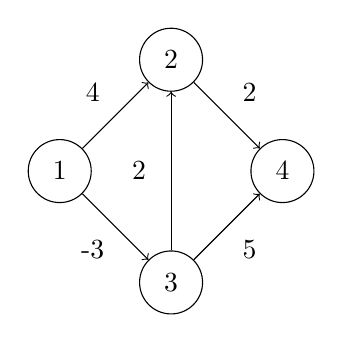
\begin{tikzpicture}[->, label/.style={draw=none}, every node/.style={shape=circle, draw, minimum size=8mm},node distance=2cm]
    \node (1) {1};
    \node (2) [above right of=1] {2};
    \node (3) [below right of=1] {3};
    \node (4) [below right of=2] {4};

    \path (1) edge node[above left, label] {4} (2) % 4
          (2) edge node[above right, label] {2} (4) % 2
          (1) edge node[below left, label] {-3} (3) % -3
          (3) edge node[left, label] {2} (2) % 2
          (3) edge node[below right, label] {5} (4); % 5
\end{tikzpicture}
                \caption{Graph mit Kantenkosten/gewichteter Graph}
                \label{fig:all-pairs-shortest-paths}
            \end{figure}

            \begin{align*}
                \delta_0(i,j) &= \begin{cases}
                    c(i, j) & \text{falls } (i, j) \in E \\
                    0 & \text{falls } i = j \\
                    \infty & \text{sonst}
                \end{cases} \\
                \delta_n(i,j) &= \delta(i,j) = \text{ Kosten des kürzesten Wehes von $i$ nach $j$}
            \end{align*}

            Frage: Wie berechnet sich $\delta_k$ aus $\delta_{k-1}$? Es gibt zwei Möglichkeiten:
            \begin{enumerate}
                \item Es kann kein neuer Knoten verwendet werden, dann: $\delta_k(i,j) = \delta_{k-1}(i, j)$
                \item Es kann ein neuer Knoten verwendet werden, dann: $\delta_k(i,j) = \delta_{k-1}(i, k) + \delta_{k-1}(k, j)$
            \end{enumerate}
            \begin{tikzpicture}[->,>=stealth',node distance=2cm, graph node/.style={circle,draw}]
            	\node[graph node] (i) {i};
            	\node[graph node] (k) [above right of=i] {k};
            	\node[graph node] (j) [below right of=k] {j};
            	
            	\path[draw, dashed]
            		(i) edge node[above left]{$\delta_{k-1} (i,k)$} (k)
            		(k) edge node[above right]{$\delta_{k-1} (k,j)$} (j);
            		
            	\path[draw]
            		(i) edge node[below]{$\delta_{k-1} (i,j)$} (j);
            \end{tikzpicture}\\
            Also:
            $$
                \delta_k(i, j) = \min\set{\delta_{k-1}(i,j), \delta_{k-1}(i, k) + \delta_{k-1}(k, j)}
            $$

            Algorithmus:
            \begin{algorithmic}
            	\For{$k\gets 1$ to $n$}
            		\ForAll{$i,j\in V$}
            			\State $\delta_k(i,j) = \min\set{\delta_{k-1}(i,j), \delta_{k-1}(i, k) + \delta_{k-1}(k, j)}$
            		\EndFor
            	\EndFor
            \end{algorithmic}
%\begin{verbatim}
%    Berechne \delta_0 nach Definition
%    for k <- 1 to n do
%        forall $i, j \in V$
%            \delta_k(i,j) = \min\set{\delta_{k-1}(i,j), \delta_{k-1}(i, k) + \delta_{k-1}(k, j)}
%    od
%\end{verbatim}


            \paragraph{Alternativ}
            $n$ mal Bellman-Ford für jeden Knoten als source $s$ durchführen.
            Laufzeit: $\LO(n \cdot n m)$.
            Besser: Übertrage Kantengewichte auf nicht negative Werte. Dann $n$ mal Dijkstra anwenden.
            Dies ergibt eine Laufzeit von $\LO(n \log n + m)$. Zur Neugewichtung der Kanten soll folgendes gelten:
            \begin{lemma}
                $\forall u, v \in V$ sei $p$ der billigste Pfad $u \to v$ mit Kantengewicht $c \in \R$.
                $\iff \forall u, v \in V$ sei $p$ der billigste Pfad $u \to v$ mit Kantengewicht  $c' \ge c$. Wähle $c'(u, v) + h(u) - h(v)$ für Funktion $h: V \to \R$.
                Dann gilt für Pfad $p = (v_0, \dots, v_k)$:
                \begin{align*}
                    c'(p) &= \sum_{i=0}^{k-1} c'(v_i, v_{i+1}) \\
                          &= \sum_{i=0}^{k-1} c(v_i, v_{i+1}) + h(v_i) - h(v_{i+1}) \\
                          &= \dots \\
                          &= c(p) + h(v_0) - h(v_k)
                \end{align*}
                Somit ergibt sich:
                \begin{align*}
                    c(p) &= \delta(v_0, v_k) \\
                    \iff c'(p) &= \delta'(v_0, v_k) &&\text{(wie $\delta$ nur mit $c'$ statt $c$)}
                \end{align*}
            \end{lemma}
            Falls $p$ Zykel $(v_0 = v_k) \implies c(p) = c'(p)$.

            Wähle $h$ so, dass alle $c' \ge 0$. Erweitere $G$ um einen Knoten $s \not\in V$ und
            die Kanten $(s, v), \forall v \in V$ mit $c(s, v) = 0$.
            Wähle $h(v) = \delta(s, v)$. Dann gilt:
            \begin{align*}
                h(v) &\le h(u) + c(u, v) \text{ für alle } (u, v) \in E \\
                \intertext{und somit:}
                0 &\le c(u, v) + h(u) - h(v) = c'(u, v)
            \end{align*}
            h wird durch einmaligen Bellman-Ford von $s$ aus in $\LO(n \cdot m)$ berechnet.




        \section{Durchmusterung von Graphen}
        Es gibt DFS (Depth-First-Search) und BFS (Breadth-First-Search).
        Bestimmung aller Knoten, die von vorgegebenem $v \in V$ erreichbar sind.
        \begin{algorithmic}
        		\State $S\gets \set{n}$
        		\State markiere alle Kanten als unbenutzt
        		\While{$\exists e\gets (u,v)\in E,\ u\in S\text{ und } (u,v)$ unbenutzt}
        			\State markiere $e$ als benutzt
        			\State $S\gets S\cup \set{v}$
        		\EndWhile
        \end{algorithmic}
%\begin{verbatim}
%    S <- {n}
%    markiere alle Kanten als unbenutzt.
%    while $\exists e = (u,v) \in E$,  $u \in S$ und $(u, v)$ unbenutzt do
%        Markiere $e$ als benutzt
%        S <- S \cup {v}
%    od
%\end{verbatim}
        Probleme:
        \begin{enumerate}
            \item Realisierung benutzt $\leftrightarrow$ unbenutzt
            \item Finden geeigneter Kanten
            \item Realisierung von $S$
        \end{enumerate}

        Lösungen:
        \begin{enumerate}
            \item Verwende Adjazenzlisten, markiere mit Trennzeiger in Liste. % Diagramma
                  Alle Knoten links davon sind benutzt, alle rechts davon unbenutzt.
            \item $\tilde S \subset S$. In \~S befinden sich alle Knoten, für die noch nicht alle Kanten gesehen wurden. (Trennzeiger noch nicht ganz rechts)
            \item Operationen: \textsc{init, insert}, $w \in S$. Lege $S$ als boolesches Feld an. Dann alle Operationen in $\LO(1)$.
                Operationen auf \~S: \textsc{init, insert}, $w \in \tilde S$, wähle $w \in \tilde S$, streichen, $\tilde S = \emptyset$?. Verwende Stack (dann ergibt sich DFS) oder Queue (dann ergibt sich BFS).
        \end{enumerate}
        
        \begin{algorithmic}
        	\Function{ExploreFrom}{Knoten s}
        		\State $S\gets \{s\}$
        		\State $\tilde S \gets \{s\}$
        		\ForAll{$v\in V$}
        			\State $p(v)\gets adjHead(v)$
        		\EndFor
        		\While{$\tilde S \not= \emptyset$}
        			\State $w\gets p(v)$, verschiebe $p(v)$
        			\If{$w\not\in S$}
        				\State\Call{Insert}{w,S}, \Call{Insert}{w,$\tilde S$}
        			\Else
        				\State \Call{Delete}{w,$\tilde S$}
        			\EndIf
        		\EndWhile
        	\EndFunction
        \end{algorithmic}

%\begin{verbatim}
%    ExploreFrom(s)
%        S <- {s}
%        S~ <- {s}
%        forall $v \in V$ do
%            p(v) <- adjHead(v);
%        od
%        while s~ != {} do
%            Sei $v \in \~S$ bel.
%            if p(v) != NIL then
%               w\gets p(v), verschiebe p(v)
%               if w\not\in S then
%               einfügen(w,S), einfügen(w,\~S)
%               else streiche (w,\~S) fi
%            fi
%        od
%\end{verbatim}

					\underline{Laufzeit}\\
					$\LO (n_s m_s)$ mit $n_s=|V_s|,\ m_s=|E_s|$, $V_s=\{v\in V|s\overset{*}{\rightarrow} v\}$\\
					(Indizierter Teilgraph $(V_s,E_s)\subseteq (V,E)$, falls $V_s\subseteq V$
					
					\begin{satz}
						Zusammenhangskomponenten können bei ungerichtetem Graphen in $\LO (n+n)$ berechnet werden.
					\end{satz}
					
%
%\begin{verbatim}
%	forall s\in V do
%	  if s\not\in S then
%	     ExploreFrom(s)
%	  fi
%\end{verbatim}					
					\begin{algorithmic}
						\ForAll{$s\in V$}
							\If{$s\not\in S$}
								\State \Call{ExploreFrom}{s}
							\EndIf
						\EndFor				
					\end{algorithmic}
					Für jede Zusammehangskomponente wird ExploreFrom 1-mal aufgerufen
										
					\subsection{Depth-First-Search (Tiefensuche)}
						bei $\tilde S$ = Keller (stack)\\
						\begin{figure}
							\centering
							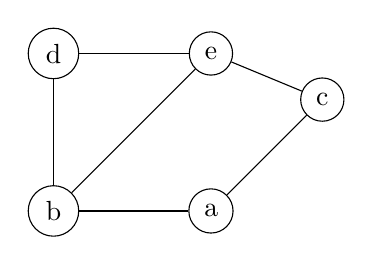
\begin{tikzpicture}[-, node distance=2cm, every node/.style={circle,draw}]
	\node (b) {b};
	\node (d) [above of=b] {d};
	\node (a) [right of=b] {a};
	\node (e) [right of=d] {e};
	\node (c) [above right of=a] {c};
	
	\path[draw]
		(b) edge (d)
		(b) edge (a)
		(b) edge (e)
		
		(d) edge (e)
		(e) edge (c)
		(c) edge (a);

\end{tikzpicture}
							\label{fig:GraphFuerSuche}
							\caption{Beispielgraph für Tiefen- und Breitensuche}
						\end{figure}
						DFS startet in a:\\
						S: a,b,d,e,c\\
						\hspace*{2cm}$\tilde S:\begin{array}{|c|}
							c\\e\\d\\b\\a\\\hline
						\end{array}$
					
					\subsection{Breadth-First-Search (Breitensuche)}
						bei $\tilde S$ = Schlange (queue)\\
						\autoref{fig:GraphFuerSuche}\\
						BFS startet in a:\\
						S: a,b,c,d,e\\
						$\tilde S$: c b a $\rightarrow$ e d c b $\rightarrow$ ...
					
					
					\subsection{DFS rekursiv}
					    $\tilde S$ als Stack.
					    \begin{algorithm}
					    		\caption{DFS}
					    		\begin{algorithmic}
					    			\Function{dfs}{Knoten v}
					    				\ForAll{$(v,w)\in E$}
					    					\If{$w\not\in S$}
					    						\State $S\gets S\cup \{w\}$
					    						\State $dfsnum(w)\gets count1,\ coun1++$
					    						\State \Call{Insert}{(v,w), T} \Comment{$(v,w)$ ist Baumkante}
					    						\State \Call{dfs}{w}
					    						\State $compnum(w)\gets count2,\ count2++$					    						
					    					\Else
					    						\If{v$\overset{*}{\underset{T}{\rightarrow}}$w}
					    							\State\Call{Insert}{(v,w),F} \Comment{$(v,w)$ ist Vorwärtskante}
					    						\Else
					    							\If{w$\overset{*}{\underset{T}{\rightarrow}}$v}
					    								\State\Call{Insert}{(v,w),B} \Comment{$(v,w)$ ist Rückwärtskante}
					    							\Else
					    								\State\Call{Insert}{(v,w),C} \Comment{$(v,w)$ ist Querkante}
					    							\EndIf
					    						\EndIf
					    					\EndIf
					    				\EndFor
					    			\EndFunction
					    		\end{algorithmic}
					    \end{algorithm}

%\begin{verbatim}
%	dfs(v)
%	for all (v,w) \in E do
%	    if w \not\in S 
%	    then 
%	        S <- S \cup {w}
%	        dfsnum(w) <- count1, count1++
%	        dfs(w)
%	        compnum(w) <- count2, count2++
%	        füge (v,w) in T hinzu
%	    else
%	        if v ->_T^* w
%	        then
%	            füge (v,w) zu F hinzu 
%	        else
%	            if w ->_T^* v
%	            then 
%	                füge (v,w) zu B hinzu
%	            else 
%	                füge (v,w) zu C hinzu
%                fi
%            fi
%        fi
%    od  
%\end{verbatim}	
                        wobei dfsnum zählt als wievielter Knoten w besucht wird und compnum sagt als wievielter Knoten w abgeschlossen wird. T ist Baumkanten und F ist Vorwärtskanten, B Rückwärtskanten, C Querkante, S die schon gesehenen Knoten. Die Notation $v \rightarrow_T^* w$ bedeutet, dass $w$ von $v$ aus über Baumkanten erreichbar ist.
                        
                        \begin{figure}[htp]
                            \centering
                            \capstart
                            \begin{tikzpicture}[->,>=stealth', every node/.style={draw, ellipse}, node distance=2cm]
	\node (a) {$a|1|6$};
	\node (b) [above of=a] {$b|2|5$};
	\node (c) [above of=b] {$c|3|1$};
	\node (d) [right of=b] {$d|4|4$};
	\node (e) [above of=d] {$e|5|3$};
	\node (f) [right of=e] {$f|6|2$};
	\node (g) [below right of=d] {$g|7|7$};
	
	\path[draw] 
		(a) edge (b)
		(b) edge (c)
		(b) edge (d)
		(d) edge[bend left] (e)
		(e) edge (f);
		
	\path[draw, dotted]
		(d) edge (f);
	
	\path[draw, densely dashed]
		(e) edge[bend left] (d);
		
	\path[draw, loosely dashed]
		(e) edge (c)
		(f) edge[bend right] (c)
		(g) edge (d);
\end{tikzpicture}
                            \caption{Rekursive Tiefensuche}
                            \label{fig:dfsrecursive}
                        \end{figure}
                        
                        \begin{lemma}
                            Sie $G=(V,E)$ ein gerichteter Graph. Es gelten
                            \begin{enumerate}
                                \item DFS auf $G$ hat lineare Laufzeit $\LO(n+m)$
                                \item $T,B,F,C$ ist Partition von $E$
                                \item $T$ entspricht dem Aufrufbaum der Rekursion
                                \item $v \rightarrow_T^* w \iff \text{dfsnum}(v) \leq \text{dfsnum}(w) \land \text{compnum}(w) < \text{compnum}(v)$
                                \item $\forall (v,w) \in E$ gilt
                                    \begin{enumerate}[a)]
                                        \item $(v,w) \in T \cup F \iff \text{dfsnum}(v) \leq \text{dfsnum}(w)$
                                        \item $(v,w) \in B \iff \text{dfsnum}(w) < \text{dfsnum}(v) \land \text{compnum}(v) < \text{compnum}(w)$
                                        \item $(v,w) \in C \iff \text{dfsnum}(w) < \text{dfsnum}(v) \land \text{compnum}(w) < \text{compnum}(v)$
                                    \end{enumerate}
                            \end{enumerate}
                        \end{lemma}
                        Aus $5.$ folgt, dass Berechnung der Partition in $T,F,B,C$ aus dfsnum/compnum folgt. Zykelfrei bedeutet, dass es keine Rückwärtskanten in $G$ gibt, d.h. $\forall (v,w) \in E : \text{compnum}(v) > \text{compnum}(w)$. Also ist $\text{num}(v) = n+1-\text{compnum}(v)$ topologische Sortierung.
                               
                \subsection{Starke Zusammenhangskomponente (SZKs)}
                    Gegeben sei ein gerichteter Graph $G = (V,E)$. Dieser heißt stark zusammenhängend, wenn es für alle $v,w \in V$ ein $v \rightarrow_E^* w$ gibt. Eine SZK von $G$ ist ein maximal stark zusammenhängender Teilgraph von $G$.
                    
                    \begin{definition}
                        Sei $(V',E')$ eine SZK. Knoten $v \in V'$ heißt Wurzel der SZK wenn 
                        $$
                            \text{dfsnum}(v) = \min\{\text{dfsnum}(w)\ : w \in V'\}
                        $$
                    \end{definition}
                    \emph{Idee:} Sei $G_{\text{aktuell}} = (V_{\text{akt}}, E_{\text{akt}})$ der von den  schon gesehenen Knoten aufgespannt wird. Verwalten die SZKs von $G_{\text{akt}}$. Am Anfang ist $V_{\text{akt}} = 1$ und $E_{\text{akt}} = \emptyset$. Betrachte Kante $(v,w)$:
                    \begin{enumerate}
                        \item $(v,w) \in T$: w kommt zu $V_{\text{akt}}$ hinzu. Bildet also eine eigene SZK
                        \item $(v,w) \not \in T$: mische eventuell mehrere SZKs zu einer
                    \end{enumerate}


%
%   Vorlesung 27.06.
%
        \subsection{Durchmustern} DFS, Berechnung von SZKs, \textsc{dfsnum}, \textsc{compnum}.

        \define{Wurzeln}{Folge von Wurzeln von nicht abg. Komp. % abgeschlossenen Komponenten?
        in aufsteigender Reihenfolge von \textsc{dfsnum}.}

        \define{Unfertig}{Folge von Knoten $v$, für die $\textsc{dfs}(v)$ aufgerufen wurde, aber SZK nicht abgeschlossen wurde. Aufsteigend nach \textsc{dfsnum}.}

        %TODO : Beispielgraph

        \paragraph{Fälle für Knoten g}
        \begin{enumerate}
            \item Kante $(g, d)$: nichts, da $d$ Abgeschlossen.
            \emph{Invariante:} Es gibt keine Kanten, die in abgschlossener Komponente starten und in nichtabgeschlossener enden.
            \item Kante $(g, h)$: $h$ ist neuer Knoten. $(g, h)$ ist Baumkante. $h$ ist neue SZK. Füge $h$ zu unfertig und Wurzeln hinzu.
            \item Kante $(g, c)$: Vereinige 3 SZKs mit Wurzeln $g, e, b$. Lösche $g, e$ aus Wurzeln.
        \end{enumerate}

        \paragraph{Algorithmus} 
        %TODO : In Algorithmusumgebung umschreiben
\begin{verbatim}
    Unfertig <- {}
    Wurzeln <- {}
    for all $v \in V$ do
        InUnfertig <- false // Boolesches Feld das Vorhandensein in Unfertig anzeigt
    od
    in dfs(v):
        push(v, Unfertig)
        InUnfertig(v) <- true
        count1 <- count1 + 1
        dfsnum(v) <- count1
        S <- S \cup {v}
        push(v, Wurzeln)
        for all (v, w) \in E do
            if w \not\in S then
                dfs(w)
            else
                if InUnfertig(w) then
                    while dfsnum(w) < dfsnum(top(Wurzeln)) do
                        pop(Wurzeln)
                    od
                fi
            fi
        od
        count2 <- count2 + 1
        compnum(v) <- count2
        if v = top(Wurzeln) then
            repeat
                w <- top(Unfertig)
                InUnfertig(w) <- false
                pop(Unfertig)
            until w = v
            pop(Wurzeln)
        fi
\end{verbatim}
        \paragraph{Laufzeit}
            Normales DFS in $\LO(n + m)$ zusätzlich wird jeder Knoten (jeweils?) einmal in \textsc{InUnfertig}, \textsc{Unfertig}, \textsc{Wurzeln} aufgenommen und gelöscht.
            $$
                \implies \LO(n + m)
            $$

    \section{Minmal aufspannende Bäume (MSTs)}
        Sei $G$ ein zusammenhängender ungerichteter Graph. Sei $c: E \to \R^+$ eine Kostenfunktion.
        %TODO : input diagram (a)
        Wollen minimal aufspannenden Teilgraph $G' = (V, E_T), E_T \subseteq E$. $G'$ zusammenhängend und $c(E_T) = \sum_{e \in E_T} c(e)$ minimal.
        \emph{Beob.:} $G'$ ist azyklisch. (Beweis durch Widerspruch). Daher: Minimal aufspannender Baum (minimum spanning tree, MST).
        %TODO : input diagram (b)

        \subsection{Kruskal-Algorithmus (Greedy)}
        \begin{enumerate}
            \item Sortiere Kanten, sodass $c(e_1) < c(e_2) < \dots < c(e_n)$.
            \item $E_T = \emptyset$, createsets(u), $V_1 \leftarrow \set{1}, V_2 \leftarrow \set{2}$
            \item
            	\begin{algorithmic}
            		\For{$i\gets 1$ to $m$}
            			\If{$(V,E_T\cup \{e_i\})$ azyklisch}
            				\State $E_T\gets E_T\cup \{e_i\}$
            			\EndIf
            		\EndFor
            	\end{algorithmic}
%\begin{verbatim}
%for i <- 1 to m do
%    if (V, E_T) \cup {e_i} azyklisch then
%        E_T <- E_T \cup {e_i}
%    fi
%od
%\end{verbatim}
        \end{enumerate}

        \begin{satz}
            Der Kruskal-Algorithmus ist korrekt.
            \begin{proof} % WAS PASSIERT HIER??
                Nenne Kantenmenge $E' \subseteq E_T$ \q{gut}, falls sie zu einem MST erweiterbar ist.
                \begin{enumerate}
                    \item \emph{Behauptung:} Sei $E' \subseteq E_T$ gut und sei $e \in E \setminus E'$ die billigste Kante, sodass $(V, E' \cup \set{e})$ azyklisch ist. Dann ist auch $E' \cup \set{e}$ gut. $\to$ Indirektion
                    \begin{proof}%[Beweis durch Widerspruch]
                        Sei $T_1 = (V, E_1)$ ein MST mit $E' \subseteq E_1$. $T_1$ existiert, da $E'$ gut. Ist $e \in E_1$, dann fertig. Falls nicht, betrachte Graph $H = (V, E_1 \cup \set{e})$. $H$ enthält einen Zykel, auf dem $e$ liegt. Da $(V, E' \cup \set{e})$ azyklisch, enthält der Zykel auch Kante aus $E_1 \setminus (E' \cup \set{e})$. Sei $e_1$ eine solche Kante. Betrachte $T_2 = (V, (E_1 \setminus \set{e_1}) \cup{e})$. $T_2$ ist aufspannend und $c(T_2) = c(T_1) + c(e) - c(e_1)$. Da $e$ billigste Kante, gilt $c(e) \le c(e_1)$ und damit $c(T_2) \le c(T_1)$. Da $T_1$ MST nach Voraussetzung, ist auch $T_2$ MST. $\implies E' \cup \set{e}$ ist gut, denn kann zu $T_2$ erweitert werden.
                    \end{proof}
                \end{enumerate}
            \end{proof}
        \end{satz}
        
        Wir ersetzen nun den Test im Algorithmus. Dies ist in \autoref{alg:kruskalUnion} beschrieben.
    	\begin{algorithm}
        		\caption{Kruskals Algorithmus mit Union-Find}
        		\label{alg:kruskalUnion}
        		\begin{algorithmic}[1]
        			\Function{Kruskal}{$G$}
        			    \For{$i \gets 1$ to $m$}
        				    \State $e_i \gets (u,v)$
        				    \State $a \gets $ \Call{Find}{$u$}
        				    \State $a \gets $ \Call{Find}{$v$}
        				    \If{$a \neq b$}
        				        \State \Call{Union}{$a,b$}
        				        \State $E_T \gets E_T \cup \set{e_i}$
        				    \EndIf
        				\EndFor
        			\EndFunction
        		\end{algorithmic}
        	\end{algorithm}
%\begin{verbatim}
%for i <- 1 to m do
%    sei e_i <- (u,v)
%    a <- Find(u)
%    b <- Find(v)
%    if a != b then
%        Union(a,b)
%        E_T <- E_T \cup {e_i}
%    fi
%od
%\end{verbatim}
        Find(u) liefert Namen der Menge in der u ist. Es gibt $2n$ Finds und $n-1$ Unions.
        
        \subsubsection{Union-Find Datenstruktur}
            \begin{enumerate}
                \item Namensfeld R[1,..,n] -> [1,..,n] wobei $R(x)$ der Name der Menge, zu der $x$ gehört. Da ergibt etwa \\
                Find(x): return R(x) \\
                Union(a,b): \\
                %TODO algorithmic
\begin{verbatim}
for i <- 1 to n do
    if R(i) = a then R(i) <- b
od
\end{verbatim}
                Damit erhält man eine Laufzeit von Find in $\LO(1)$ und Union in $\LO(n)$. Gesamt also $\LO(m+n^2üm \log m)$
            \end{enumerate}   
            Wir wollen nun den Union von $\LO(n)$ so verbessern, dass er nicht alle Elemente besucht.  Merke für jede Menge die Elemente, die dort enthalten sind. Behalte bei Union immer den Namen der größeren Menge. Benötigte Funktionen sind nun in \autoref{alg:unionFind} dargestellt. Worst case Union: $\LO(n), \abs{a} = \frac{n}{2}, \abs{b} = \frac{n}{2}$. 
    	\begin{algorithm}
        		\caption{Funktionen für Union-Find}
        		\label{alg:unionFind}
        		\begin{algorithmic}[1]
        			\Function{createSet}{}
        			    \For{$i \gets 1$ to $n$}
        				    \State \Call{R}{x} $ \gets x$ \Comment{Speichert Wurzel des Baumes}
                            \State \Call{Elem}{x} $ \gets x$ \Comment{Speichert Elemente des Baums}
                            \State \Call{Size}{x} $ \gets x$
                        \EndFor
        			\EndFunction
        			\Statex
        			\Function{Find}{$x$}
        			    \State \Return \Call{R}{$x$}
        			\EndFunction
        			\Statex
        			\Function{Union}{$a,b$}
        			    \If{\Call{size}{$a$} $<$ \Call{size}{$b$}} \Comment{$a$ muss größer/gleich $b$ sein}
        			        \State \Call{Swap}{$a,b$}
        			    \EndIf
        			    \ForAll{$x \in $ \Call{Elem}{$b$}}
        			        \State \Call{R}{x} $ \gets a$  
        			        \State $e_a \gets $ \Call{Elem}{$a$} 
        			        \State \Call{Insert}{$x,e_a$}
        			    \EndFor
        			\EndFunction  
        		\end{algorithmic}
        	\end{algorithm}
%\begin{verbatim}
%createSet:
%for x <- 1 to n do
%    R(x) <- x
%    elem(x) <- x
%    size(x) <- 1
%    
%Find(x): 
%return r(x)
%
%Union(a,b)
%if size(a) < size(b) then vertausche(a,b)
%for all x \in Elem(b)
%    R(x) <- a
%    insert(x, Elem(a))
%od
%\end{verbatim}                       
            \begin{satz}
                Mit der beschriebenen Struktur können createset, $n-1$ Unions und $2n$ Finds in Zeit $\LO(n \log n + m)$ ausgeführt werden.
            \end{satz}        
            
            \begin{proof}
                Createset und $2m$ Finds gehen in $\LO(n+m)$. Wir Behaupten nun, dass $n-1$ Unions $\LO(n \log n)$ kosten. Ein Union(a,b) vereinigt zwei Mengen mit $n_a, n_b$ Elementen. Sei $n_b < n_a$, dann folgt eine Laufzeit von $\LO(1 + n_b)$. Damit haben wir eine Gesamtzeit von $\LO(\sum_{i=1}^{n-1}{n_i+1})$ mit $n_i$ Größe der kleineren Menge beim $i$-ten Union. Wechselt ein Element die Menge, so trängt es $1$ zu $n_i$ bei. Element $j$ wechselt $r_j$ die Menge. Es gilt also
                $$
                    \sum_{i=1}^{n-1}{n_i}  = \sum_{j=1}^{n-1}{r_j}
                $$ 
                Behauptung: $r_j \leq \log n$ für alle Knoten $j$
                \begin{proof}
                    Wenn $j$ in Menge mit $l$ Elementen ist und wechselt, dann kommt $j$ in eine Menge der Größe $\geq 2l$. Das heißt beim $k$-ten Wechsel ist $j$ in Menge mit mindestens $\geq 2^k$ Elementen. Da es nur $n$ Elemente gibt gilt $2^k \leq n$ und daraus folgt $k \leq \log n$
                \end{proof}
                Insgesamt folgt nun
                $$
                    \sum_{i=1}^{n-1}{n_i}  = \sum_{j=1}^{n-1}{r_j} = n \log n    
                $$
                Damit ist die Laufzeit für Kruskals Algorithmen $\LO(m \log n)$
            \end{proof}
            
    \subsection{Union-Find}
        Halte für jede Menge Baum. Damit geht Union in $\LO(1)$. Für Find läuft man im Baum hoch zur Wurzel. Das geht in $\LO(\text{Tiefe}(\text{Baum}))$. Für weitere Verbesserungen führe folgende Optimierungen ein
        \begin{enumerate}
            \item Gewichtete Verinigungsregel: Hänge kleinen an großen Baum
            \item Pfadkomprimierung: Laufe Pfad hoch. Hänge alle Zeiger auf Wurzel
        \end{enumerate}   
        \begin{satz}
            n Unions + m Finds gehen in Zeit $\LO(n + m \cdot \alpha (m+n,n))$ wobei $\alpha$ invers zur Ackermannfunktion ist. Das ist kleiner als 5 für alle realistischen Werte.
        \end{satz}          
            
            
    \subsection{PRIMs Algorthmus}
        Beschrieben in \autoref{alg:prim}. Dabei liegen in $E_T$ die Kanten des Spannbaums. Korrektheitsbeweis analog zu vorher: Induktiv über gute Erweiterungen.
    	\begin{algorithm}
        		\caption{Prims Algorithmus}
        		\label{alg:prim}
        		\begin{algorithmic}[1]
        			\Function{Prim}{$G$}
        			    \State $T \gets \set{v}$
        				\While{$T \neq \set{V}$}
        				    \State $e \gets (u,w) \in E \text{ mit } u \in T \land w \not \in T \text{ und } c(e) \text{ minimal}$
        				    \State $E_T \gets E_T \cup \set{e}$
        				    \State $T \gets T \cup \set{w}$
        				\EndWhile
        			\EndFunction
        		\end{algorithmic}
        	\end{algorithm}
%\begin{verbatim}
%t <- {v}
%while T != {V} do
%    sei e = (u,w) \in E mit u \in T und w \not \in T 
%        mit c(e) minimal
%    E_T <- E_t \cup {e}
%    T <- T \cup {w}
%od
%\end{verbatim}
        
        
        \subsubsection{Laufzeit}
            Priority Queue mit Schlüsseln $\set{c(w) | w \not \in T \land c(w) = \min\set{c(u,w),u \in T}}$. Suche $w$ mit kleinstem $c(w)$, entspricht deleteMin bei Dijkstra. Wird $w$ in $T$ eingefügt, so tue für alle $(w,x) \in E$ mit $x \not \in T$ und $c(x) \leftarrow \min \set{c(x), c(w,x)}$. Das entspricht DecreasyKey bei Dijkstra. 
            
        \subsubsection{Implementierung}
            Priority Queue als primären Heap. Dabei gehen Operationen in $\LO(\log n)$. Insgesamt also $\LO(m \log n)$. Statt bin. Heap verwende (a,b)-Baum mit $ a = \max(2,\frac{m}{n})$ und $b=2a$. Damit ergibt sich eine Laufzeit von $\LO(m \frac{\log n}{\log \frac{m}{n}})$ Das ist gut, wenn $m$ etwa $n^2$ ist.
            
    
        
     \section{Zweifach Zusammenhangs Komponente von ungerichteten Graphen}
        Graph heißt 2-fach zusammenhängend, falls $G-\{v\}$\footnote{$G'=\left(V\backslash\{v\},\left(E\backslash\{(v,x)\forall x\in V\}
        \right)\backslash\{(x,v)\forall x\in V\}\right)$} zusammenhängend für alle $v\in V$\\
        Eine 2ZK ist maximal 2-fach zusammenhängender Teilgraph. $v\in V$ heißt Artikulationspunkt, wenn $G-\{v\}$ nicht zusammenhängend\\
        
        %TODO Zeichnung

        2ZK's: $\{1,2\},\{6,7\},\{2,3,4\},\{4,5,6\}$\\
        Artikulationspunkte: $2,4,6$
        
        \subsection{DFS für ungerichtete Graphen}
        	Es gibt Baumkanten T und Rückwärtskanten B, jedoch keine Vorwärts- und Querkanten.\\\\
        	\emph{Idee:}\\
        		v ist kein Artikulationspunkt, falls ein Baumnachfolger w von v eine Rückwärtskante ''vor'' v hat\\
        		x ''vor'' v $\Leftrightarrow dfsnum(x)<dfsnum(v)$\\
        		Falls v Wurzel des dfs-Baumes und mehrere Zweige, so ist v Artikulationspunkt.
        	\begin{definition}
        		$low(u)\gets \min\{dfsnum(u);\min\{dfsnum(v)$ mit Pfad $u\overset{*}{\underset{T}{\rightarrow}}Z\rightarrow v\}\}$
        	\end{definition}
        	\begin{algorithm}
        		\caption{Tiefensuche auf ungerichteten Graphen}
        		\begin{algorithmic}[1]
        			\Function{dfs}{Knoten v}
        				\ForAll{$(v,w)\in E$)}
        					\If{w unbesucht}
        						\State $dfsnum(w)\gets count$; $count++$
        						\State $low(w)\gets dfsnum(w)$
        						\If{$low(w)<low(v)$}
        							\State $low(v)\gets low(w)$
        						\EndIf
        						\If{$low(w)>dfsnum(v)$}
        							\State $artpunkt(v)\gets TRUE$
        						\EndIf
        					\Else
        						\If{$dfsnum(w)<low(v)$}
        							\State $low(v)\gets dfsnum(w)$
        						\EndIf
        					\EndIf
        				\EndFor
        			\EndFunction
        		\end{algorithmic}
        	\end{algorithm}
        	In (7) wird low-Wert von w an low(v) übergeben, falls er kleiner ist\\
        	In (14) wird Rückwärtskante von v nach w berücksichtigt\\
        	In (10) wird erkannt, ob der Zweig, der aus v in Richtung w startet keine Rückwärtskante ''vor'' v enthält $\Rightarrow$ v ist Artikulationspunkt\\\\
        	\emph{Laufzeit:} $\mathcal{O}(n+m)$ (Verfeinerung von DFS)\\\\
        	\emph{Spezialfall:} v Wurzel
        	\begin{algorithmic}
	        	\If{$dfsnum(v)==1 \&\& \exists w_1\not= w_2\text{ mit }(v,w_1),(v,w_2)\in T$}
	        		\State $artpunkt(v)\gets TRUE$
	        	\EndIf
        	\end{algorithmic}
        	\emph{Was fehlt:} Berechnung der 2ZK wenn Artikulationspunkte gegeben ($\rightarrow$ Übung)
        	
    \section{EXKURS: Stable Marriage}
		Vollständiger bipartiter Graph aus n Männern und n Frauen.\\
		Jede Person hat Rangliste $\{0,...,n-1\}$ für das andere Geschlecht:
		\begin{itemize}
			\item $w(x,Y)$ Gewicht von Mann aus gesehen
			\item $w(Y,x)$ Gewicht von Frau aus gesehen
		\end{itemize}
		%TODO Beispielgraph
		(a,A),(b,B),(c,C) nicht stabil:\\
		c findet B attraktiver als C und B findet c attraktiver als b\\\\
		
		Suche perfektes Matching M, sodass es kein $(x,Y),(Y,x)$ mit $w(x,Y)>w(x,X)$ und $w(Y,x)>w(Y,y)$
		
		\subsection{Algorithmus}
			Alle Männer sind frei.\\
			Wähle einen freien Mann, der wählt seine beste Frau, die ihn noch nicht abgelehnt hat. Diese akzeptiert oder lehnt ab, je nachdem ob das Angebot ihren Status verbessert.\\
			Evtl. wird ihr bisheriger Mann frei.\\
			Es gilt: Verheiratete Frauen bleiben verheiraten, aber nicht unbedingt mit demselben Mann
			\subsubsection{Termination}
				Alle Frauen bekommen irgendwann ein Angebot, bleiben ab dann verheiratet.\\
				\emph{Männersicht:}\\
					Macht Mann n Angebote haben vorher $n-1$ abgelehnt. Diese letzte muss frei sein, diese akzeptiert.
			\subsubsection{Korrektheit}
				Es gibt \emph{kein} (x,X)(y,Y), wo x Y attraktiver findet als X (x hat Y vor X gefragt) \emph{und gleichzeitig} Y x attraktiver findet als y (denn Y hatte x abgelehnt)
			\subsubsection{Laufzeit}
				$\LO\left(\sum\limits_{i=1}^n i\right)=\LO(n^2)$\footnote{$\rightarrow$ Buch: Kleinberg/Tardos}
				\paragraph{Frage:}
					Erwartete Laufzeit, wenn Referenzen der Männer zufällig sind, die der Frauen beliebig aber fest.\\
					\emph{Idee:}\\
					Jeder Mann wählt seine Präferenz nach und nach (wenn er sie braucht).
					x macht immer einer zufälligen Frau ein Angebot, der er noch kein Angebot gemacht hat oder einfach: Er wählt \emph{immer eine} zufällige Frau.\\
					Wann haben alle Frauen mind. 1 Angebot?\\
					$\rightarrow$ ''Coupon Collector Problem''
		\subsection{Coupon Collector Problem - Laufzeit}
			Wie viele Bälle müssen auf n Körbe geworfen werden, bis jeder Korb $\geq 1\times$ getroffen ist?\\
			
			Ergebnis: $\Theta(n\log n)$\\
			
			$P(\text{Korb i nach k Würfen nicht getroffen})=\left( 1-\frac{1}{n}\right)^k\approx e^{-\frac{k}{n}}$\\
			Mit $k=c\cdot n$: $P(\text{Korb i nach k Würfen nicht getroffen})=e^{-c}$\\
			Mit $k=c\cdot n\log n$: $P=e^{-c\cdot \log n}=\left(\frac{1}{n}\right)^c$\\\\
			$\Rightarrow$ Mit hoher Wahrscheinlichkeit ist nach $(c-1)\cdot n\log n$ Versuchen kein Korb leer. Wähle $c>1$.
			
        	